% !TeX root = er.tex

\chapter{Unidades de medida}\label{ch.units}

As tabelas~\ref{tab.units} e \ref{tab.prefixes} mostram as unidades de medida e suas abreviações.

\begin{table}
\caption{Unidades de medida}
\label{tab.units}
\begin{tabular}{p{2cm}p{1.5cm}p{2.5cm}p{2cm}}
\hline\noalign{\smallskip}
Propriedade & Variável & Unidade & Abreviação\\
\noalign{\smallskip}\hline\noalign{\smallskip}
Distance & $s$ & meter  & m\\
Time &  $t$ & second & s\\
Velocity & $v$ & meter/second &  m/s\\
Acceleration & $a$ & meter/second$^2$ & m/s$^2$\\
Frequency & $f$ & hertz & Hz\\
Angle & $\theta$ & radian & rad\\
& & degree & $^\circ$\\
\noalign{\smallskip}\hline\noalign{\smallskip}
\end{tabular}
\end{table}

\begin{table}
\caption{Prefixos}
\label{tab.prefixes}
\begin{tabular}{p{1.5cm}p{2.2cm}p{1.7cm}}
\hline\noalign{\smallskip}
Prefixo & Significado & Abreviação \\
\noalign{\smallskip}\hline\noalign{\smallskip}
kilo- & thousands & k\\
centi- & hundreths & c\\
milli- & thousandths & m\\
micro- & millionths & $\mu$\\
\noalign{\smallskip}\hline\noalign{\smallskip}
\end{tabular}
\end{table}

\noindent\textbf{Exemplos:}

\begin{itemize}\setlength{\itemsep}{6pt}
\item $20$ kHz $=$ $20$ kilohertz $=$ $20,000$ hertz
\item $15$ cm $=$ $15$ centimeters $=$ $\frac{15}{100}$ meters
\item $50$ ms $=$ $50$ milliseconds $=$ $\frac{50}{1000}$ seconds
\item $10$ $\mu$s $=$ $10$ microseconds $=$ $\frac{10}{1000}$ milliseconds $=$ $\frac{10}{1000000}$ seconds
\end{itemize}

Os ângulos, como o rumo de um robô e a direção para um objeto, são medidos em graus ou radianos (Fig.~\ref{fig.angles}). Por convenção, os ângulos são positivos no sentido anti-horário e negativos no sentido horário, conforme medido a partir da frente do robô.

\begin{figure}
\begin{center}
% The unit circle divided into 45 degree segments
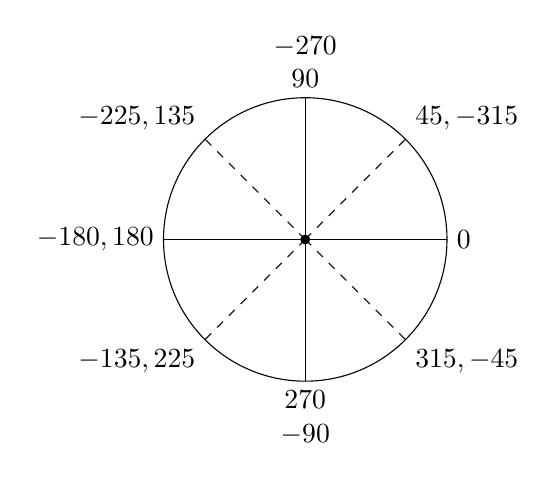
\begin{tikzpicture}[scale=1.8]
\coordinate (origin) at (0,0);
% Draw circle
\draw (origin) circle [radius=1];
% Draw axes
\draw (-1,0) node [left] {$-180,180$} -- (1,0) node [right] {$0$};
\draw (0,-1) node [below,align=flush center] {$270$\\$-90$} -- (0,1) node [above,align=flush center] {$-270$\\$90$};
% Draw other angles
\draw[dashed] (origin) -- +(45:1) node[above right] {$45,-315$};
\draw[dashed] (origin) -- +(135:1) node[above left] {$-225,135$};
\draw[dashed] (origin) -- +(225:1) node[below left] {$-135,225$};
\draw[dashed] (origin) -- +(315:1) node[below right] {$315,-45$};
% Dot at origin
\fill (origin) circle [radius=1pt];
\end{tikzpicture}

\bigskip
\bigskip

% The unit circle with radians divided into pi/4 segments
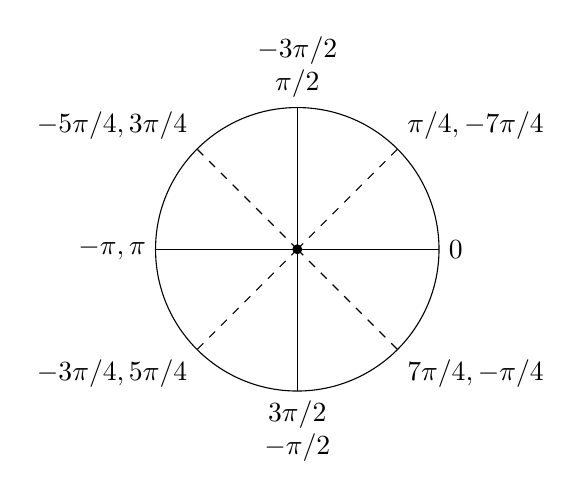
\begin{tikzpicture}[scale=1.8]
\coordinate (origin) at (0,0);
% Draw circle
\draw (origin) circle [radius=1];
% Draw axes
\draw (-1,0) node [left] {$-\pi,\pi$} -- (1,0) node [right] {$0$};
\draw (0,-1) node [below,align=flush center] {$3\pi/2$\\$-\pi/2$} -- (0,1) node [above,align=flush center] {$-3\pi/2$\\$\pi/2$};
% Draw other angles
\draw[dashed] (origin) -- +(45:1) node[above right] {$\pi/4,-7\pi/4$};
\draw[dashed] (origin) -- +(135:1) node[above left] {$-5\pi/4,3\pi/4$};
\draw[dashed] (origin) -- +(225:1) node[below left] {$-3\pi/4,5\pi/4$};
\draw[dashed] (origin) -- +(315:1) node[below right] {$7\pi/4,-\pi/4$};
% Dot at origin
\fill (origin) circle [radius=1pt];
\end{tikzpicture}
\end{center}

\caption{Ângulos em graus (acima) e radianos (abaixo)}\label{fig.angles}
\end{figure}

\chapter{Derivações matemáticas e tutoriais}\label{ch.math}

Este apêndice reúne as derivações matemáticas utilizadas no texto, bem como pequenos tutoriais de conceitos que podem não ser familiares.

\section{Probabilidade condicional e Bayes governam}\label{a.bayes}

Dada uma leitura de $z$ do sensor, qual é a probabilidade de que estejamos na posição $x_i$? Isto é expresso como uma \emph{probabilidade condicional} $p(x_i)\mid z)$. Os dados que temos disponíveis são a probabilidade \emph{current} $p(x_i)$ de estarmos a $x_i$, e $p(z\mid x_i)$, a probabilidade condicional de o sensor ler $z$ se estivermos de fato a $x_i$. Vamos multiplicar estas duas probabilidades:
\[
p(z\mid x_i)\, p(x_i)\,.
\]
O que isso significa? O evento $x_i$ ocorre com probabilidade $p(x_i)$ e uma vez que ocorre o evento $z$ ocorre com probabilidade $p(z\mid x_i)$. Portanto, esta é a probabilidade de que ambos $z$ e $x_i$ ocorram, chamada de \emph{probabilidade conjunta} dos dois eventos:
\[
p(z \cap x_i) = p(z\mid x_i)\, p(x_i)\,.
\]
A probabilidade conjunta também pode ser obtida multiplicando a probabilidade condicional por $x_i$ dado $z$ pela probabilidade de $z$:
\[
p(x_i \cap z) = p(x_i\mid z)\, p(z)\,.
\]
A probabilidade conjunta é comutativa, portanto, equacionando as duas expressões que temos:
\[
p(x_i\mid z)\, p(z) = p(x_i \cap z) = p(z \cap x_i) = p(z\mid x_i)\, p(x_i)\,.
\]
Dividir por $p(z)$ dá:
\[
p(x_i\mid z)= \frac{p(z\mid x_i)\, p(x_i)}{p(z)}\,,
\]
que é conhecido como \emph{Bayes rule}.

Se soubermos $p(z)\mid x_i)$ e $p(x_i)$ para cada $i$, $p(z)$, a \emph{probabilidade total} do evento $z$, pode ser calculada pela soma das probabilidades individuais conhecidas:
\begin{displaymath}
p(z) = \sum_i p(z\mid x_i)\, p(x_i)\,.
\end{displaymath}

\noindent\textbf{Exemplo} Façamos o cálculo para o exemplo em Sect.~\ref{s.prob-local}. Que $x_i$ seja o evento em que estamos na posição $i$ e que $z$ seja o evento em que o robô detecta uma porta. Inicialmente, $p(x_i)=.125$ para todas as posições $x_i$, e, se o robô estiver em uma porta, a probabilidade de que o sensor detecte isto corretamente é $.9$, enquanto a probabilidade de que ele detecte uma porta incorretamente é $1-.9=.1$. A probabilidade de detectar uma porta, $p(z)$, é obtida pela soma das probabilidades em cada posição, onde a probabilidade é $,125\times 0,9 = .1125$ em uma posição com uma porta e $,125\times .1= .0125$ em uma posição sem porta:
\[
p(z)=.1125 + .1125 + .0125 + .0125 + .1125 + .1125 + .1125 + .0125 = .575\,.
\]
Pela regra de Bayes, a probabilidade de estar na posição $i$ com uma porta \emph{se} é detectada:
\[
p(x_i \mid z) = \frac{p(z\mid x_i)\, p(x_i)}{p(z)}=\frac{.9\times .125}{.575} = .196\,,
\]
enquanto a probabilidade de estar na posição $i$ sem porta, mas uma porta é detectada de forma incorreta:
\[
p(x_i \mid z) = \frac{p(z\mid x_i)\, p(x_i)}{p(z)}=\frac{.1\times .125}{.575} = .022\,.
\]

\section{Normalização}\label{a.normalize}

O conjunto de probabilidades dos possíveis resultados de um evento deve somar até $1$, uma vez que um dos resultados deve ocorrer. Se uma porta for detectada, o robô deve estar em uma das posições de $8$ possíveis, mas a soma sobre todas as posições de $i$ da probabilidade de que o robô esteja na posição de $i$ foi mostrada acima:
\[
.1125 + .1125 + .0125 + .0125 + .1125 + .1125 + .1125 + .0125 = .575\,.
\]
As probabilidades devem ser {normalizadas} através da divisão pela soma de $,575$ para que a soma seja de $1$. As probabilidades normalizadas são de $.1125/.575 \approx .19$ e $.0125/.575 \approx .02$, que somam até $1$:
\[.19 + .19 + .02 + .02 + .19 + .19 + .19 + .02 \approx 1\,.\]

\section{Média e variância}\label{a.mean}

O \emph{média}\footnote{\textit{Mean} é o termo técnico para a média.} $\mu$ de um conjunto de valores $\{x_1,\ldots,x_n\}$ é:
\[
\mu = \frac{1}{n}\sum^n_{i=1} x_i\,.
\]
Considere cinco pessoas que ganham $8,9,10,11,12$ mil Euros por ano, respectivamente. Seu salário médio é:
\[
\mu = \frac{8+9+10+11+12}{5} = \frac{50}{5} = 10\,.
\]
A média não nos diz muito porque a mesma média pode ser obtida a partir de dados muito diferentes:
\[
\mu = \frac{5+6+10+14+15}{5} = \frac{50}{5} = 10\,.
\]
A média é significativamente influenciada por \emph{outliers}: valores que são muito superiores ou inferiores aos demais valores. Se a pessoa que ganha $10$ mil Euros de repente recebeu um bônus de $90$ mil Euros, o salário médio é agora:
\[
\mu = \frac{8+9+100+11+12}{5} = \frac{140}{5} = 28\,.
\]
Um político saltaria a oportunidade de afirmar que, durante seu mandato, o salário médio havia subido em $180\%$!

\emph{Variância} é uma medida da propagação de um conjunto de valores. Quanto mais próximos estiverem os valores, mais baixa será a variância. Medidas como a média são mais confiáveis se os valores estiverem agrupados e, portanto, tiverem uma baixa variância. A fórmula para a variância de um conjunto de valores $\{x_1,\ldots,x_n\}$ é:\footnote{$n-1$ conta os \emph{graus de liberdade}. Como a média é calculada antes da variância, não podemos escolher os valores $n$ arbitrariamente; o último valor escolhido é obrigado a ser o valor que faz com que o cálculo produza a média dada.}
\[
s^2 = \frac{1}{n-1}\sum^n_{i=1} (x_i-\mu)^2\,.
\]
Cada termo $x_i-\mu$ mede a distância do valor $x_i$ da média; a variância é a média dos quadrados dessas distâncias. As distâncias são quadradas para que os valores de cada lado da média não se anulem mutuamente. Por exemplo, dados os valores $100$ e $300$, sua média é $200$; se computássemos a variância como $(100-200)+(200-300)$, o resultado seria $0$ mesmo que os valores estejam dispersos. Usando a definição acima, a variância é $(100-200)^2+(200-300)^2=20000$.

Para o conjunto de dados $ 8,9,10,11,12$ a variação é:
\[
s^2 = \frac{(-2)^2+(-1)^2+0+1^2+2^2}{5-1} = \frac{10}{4} = 2.5\,,
\]
while for the data set $\{5,6,10,14,15\}$ the variance is:
\[
s^2 = \frac{(-5)^2+(-4)^2+0+4^2+5^2}{4} = 20.5\,.
\]
Como $20,5$ é muito maior que $2,5$, os dados do segundo conjunto estão distribuídos em uma faixa mais ampla que os dados do primeiro conjunto. Depois que o bônus é recebido, a variação é:
\[
s^2 = \frac{20^2+19^2+72^2+17^2+16^2}{4} = \frac{6490}{4} = 1622.5\,.
\]
Claramente, não se deve interpretar o salário médio como significativo se houver outliers.

\section{Covariância}\label{a.covariance}

Considere um grupo de dez pessoas que ganham os seguintes salários:
\[x_1=\{11,12,13,14,15,16,17,18,19,20\}\,,
\]
em milhares de euros. O salário médio é:
\[
\mu_1=\frac{1}{10}(11+12+13+14+15+16+17+18+19+20)=15.5\,.
\]
Conjecturamos que as pessoas com salários mais altos compram carros mais caros do que aquelas com salários baixos. Suponha que haja dois modelos de carros sendo vendidos naquela área, um por $10$ mil Euros e outro por $20$ mil Euros. O conjunto de dados a seguir mostra os carros comprados por este grupo de pessoas, onde o elemento $i$'th é o custo do carro comprado pela pessoa de $i$'th:
\[
x_2=\{10,10,10,20,10,20,10,10,20,20\}\,.
\]
Para ver se existe alguma conexão entre os salários e os custos dos carros, calcula-se o \emph{covariância} $\textit{cov}(x_1,x_2)$ entre os conjuntos de dados $x_1$ e $x_2$. O cálculo é semelhante ao da variância, exceto que ao invés de quadriplicar a diferença entre um valor em um único conjunto e a média desse conjunto, multiplicamos a diferença entre um valor do primeiro conjunto e sua média pela diferença entre um valor do segundo conjunto e sua média:
\[
\textit{cov}(x_1,x_2) = \frac{1}{n-1}\sum^n_{i=1} (x_{1,i}-\mu_1)(x_{2,i}-\mu_2)\,.\label{eq.cov}
\]
A covariância dos conjuntos de valores $x_1$ e $x_2$ é de $7,8$, um valor positivo, o que indica que os salários e o custo do carro aumentam juntos, ou seja, as pessoas que ganham mais dinheiro tendem a comprar carros mais caros. Se as cinco primeiras pessoas comprarem carros no valor de $10$ e as cinco seguintes comprarem carros no valor de $20$, a covariância se torna de $13,9$, indicando uma conexão mais forte entre o salário e o custo de um carro. Por outro lado, se os cinco primeiros comprarem carros caros e os cinco seguintes comprarem carros baratos, a covariância é de $-13,9$, de modo que, conforme o salário sobe, o custo de um carro desce. Finalmente, se todos comprarem o mesmo carro, a covariância é de $0$ e concluímos, como esperado, que não há conexão entre o salário de um e o carro que se compra.

A covariância é simétrica porque a multiplicação dos números reais é comutativa:
\begin{eqnarray*}
\textit{cov}(x_1,x_2) &=& \frac{1}{n-1}\sum^n_{i=1} (x_{1,i}-\mu_1)(x_{2,i}-\mu_2)\\
&=& \frac{1}{n-1}\sum^n_{i=1} (x_{2,i}-\mu_2)(x_{1,i}-\mu_1)\\
&=&\textit{cov}(x_2,x_1)\,.
\end{eqnarray*}

A matriz de covariância combina as variações e as covariâncias:
\[
\left[ \begin{array}{ll} s^2(x_1) & \textit{cov}(x_1,x_2)\\ \textit{cov}(x_2,x_1)& s^2(x_2)\end{array}\right]\,.
\]
$\textit{cov}(x_1,x_2)=\textit{cov}(x_2,x_1)$, so there are only three valores diferentes na matriz.

\section{Multiplicação de vetores e matrizes}\label{a.matrices}

Multiplicação de uma matriz (bidimensional) $\vec{M}$ por um vetor $\vec{v}$ dá um novo vetor:
\[
\spacearray
\vec{M}\vec{v}=\left[ \begin{array}{c} a\\c\end{array} \begin{array}{c} b\\d \end{array}\right]\, \left[ \begin{array}{c} x\\y\end{array}\right] = \left[ \begin{array}{c} ax+by\\cx+by\end{array}\right]\,.
\]
A multiplicação de duas matrizes é feita multiplicando as linhas da matriz esquerda separadamente com cada vetor de coluna da matriz direita para obter os vetores de coluna para a matriz resultante:
\[
\spacearray
\left[ \begin{array}{c} a\\c\end{array} \begin{array}{c} b\\d \end{array}\right]\, \left[ \begin{array}{c} x\\y\end{array} \begin{array}{c} u\\v\end{array}\right] = \left[ \begin{array}{c} ax+by\\cx+dy\end{array} \;\; \begin{array}{c} au+bv\\cu+dv\end{array}\right]\,.
\]
A matriz identitária é:
\[
\spacearray
\vec{I}=\left[\begin{array}{c} 1\\0\end{array} \begin{array}{c} 0\\1\end{array}\right]
\]
e é fácil de verificar que para qualquer matriz $\vec{M}$, $\vec{M}\, \vec{I} = \vec{I}\, \vec{M} = \vec{M}$.
Para uma matriz $\vec{M}$, seu inverso $\vec{M}^{-1}$ é a matriz que resulta em $\vec{I}$ quando multiplicado por $\vec{M}$:
\[
\spacearray
\vec{M}=\left[ \begin{array}{c} a\\c\end{array} \begin{array}{c} b\\d \end{array}\right]\,,\;\;\;\;
\vec{M}^{-1}=\frac{1}{\textit{det}\,(\vec{M})}\left[ \begin{array}{c} d\\-c\end{array} \begin{array}{c} -b\\a \end{array}\right]\,,
\]
onde $\textit{det}\,(\vec{M})$, o \emph{determinante} de $\vec{M}$, é $ad-bc$. Podemos verificar isso multiplicando:
\[
\spacearray
\left[ \begin{array}{c} a\\c\end{array} \begin{array}{c} b\\d \end{array}\right] \cdot
\left[ \begin{array}{c} d\\-c\end{array} \begin{array}{c} -b\\a \end{array}\right] =
\left[ \begin{array}{c} ad-bc\\cd-dc\end{array} \;\;\begin{array}{c} -ab+ba\\-bc+da \end{array}\right] =
\left[ \begin{array}{c}ad-bc \\0\end{array}\;\; \begin{array}{c} 0\\ad-bc \end{array}\right]\,.
\]
Isto é válido somente para matrizes cujo determinante não é zero, porque as matrizes \emph{singulares} - aquelas cujo determinante é zero - não têm um inverso.

\section{A área de um trapézio na base de um triângulo}\label{a.trap}

O diagrama seguinte mostra um triângulo de largura $w$ e altura $h$ com uma linha paralela à altura $h'$ que cria um trapézio:

\begin{center}
% Computing the area from the uncertainty
\begin{tikzpicture}[scale=1.3]
\draw (0,0) -- (1.5,3) -- (3,0) -- node[below] {$w$} cycle;
\draw (.5,1) -- node[below] {$w'$} (2.5,1);
\draw[<->] (-.4,0) -- node[left] {$h$} (-.4,3);
\draw[<->] (3.4,0) -- node[right] {$h'$} (3.4,1);
\draw[<->] (3.4,1) -- node[right] {$h-h'$} (3.4,3);
\end{tikzpicture}
\end{center}

Queremos encontrar uma fórmula para a área do trapézio usando os valores $w, h, h'$. A área $a$ é a diferença entre as áreas dos dois triângulos:
\begin{displaymath}
a = \frac{wh}{2} - \frac{w'(h-h')}{2}\,.
\end{displaymath}
Por triângulos semelhantes:
\begin{displaymath}
\frac{h}{h-h'} = \frac{w}{w'}\,,
\end{displaymath}
portanto:
\begin{displaymath}
w' = \frac{w(h-h')}{h}\,.
\end{displaymath}
Substituição:
\begin{eqnarray*}
a &=& \frac{wh}{2} - \frac{w(h-h')(h-h')}{2h}\\[8pt]
&=&\frac{w(h^2-(h-h')^2)}{2h}\\[8pt]
&=&\frac{w(h^2-h^2+2hh'-h'^2)}{2h}\\[8pt]
&=&\frac{w(2hh'-h'^2)}{2h}\\[8pt]
&=&wh'(1-\frac{h'}{2h})\,.
\end{eqnarray*}

\section{Fórmulas algébricas para $\cos 15^{\circ}$}\label{a.cosine}

O Eq.~\ref{eq.cos15} afirma que:
\[
\cos^{-1}\left(\frac{\sqrt{2+\sqrt{3}}}{2}\right) = \pm 15^{\circ}\,.
\]
Usando a fórmula para o cosseno da diferença de dois ângulos, nós temos:
\begin{eqnarray*}
\cos 15^\circ &=& \cos(45^\circ-30^\circ)\\
&=& \cos 45^\circ \cos 30^\circ + \sin 45^\circ \sin 30^\circ\\
&=&\frac{\sqrt{2}}{2}\cdot \frac{1}{2} + \frac{\sqrt{2}}{2}\cdot \frac{\sqrt{3}}{2}\\
&=&\frac{\sqrt{2}+\sqrt{6}}{4}\,.
\end{eqnarray*}
Agora calculamos:
\[
\left(\frac{\sqrt{2}+\sqrt{6}}{4}\right)^2 =
\left(\frac{8+2\sqrt{2}\sqrt{6}}{16}\right)=\frac{2+\sqrt{3}}{4}=
\left(\frac{\sqrt{2+\sqrt{3}}}{2}\right)^2\,.
\]
